\section{Lengths of Curves}
If we're at some point $(x,f(x))$ and move $\d{x}$ units over, we'll be at a new point $(x+\d{x},f(x+\d{x}))$.
This point is $\d{x}$ units horizontally and $\d{y}=f(x+\d{x})-f(x)$ vertically away from $(x,f(x))$.
So, by the Pythagorean Theorem, the new point is $\d{s} = \sqrt{(\d{x})^2+(\d{y})^2}$ units away.

\begin{figure}[H]
	\label{arclength}
	\centering
	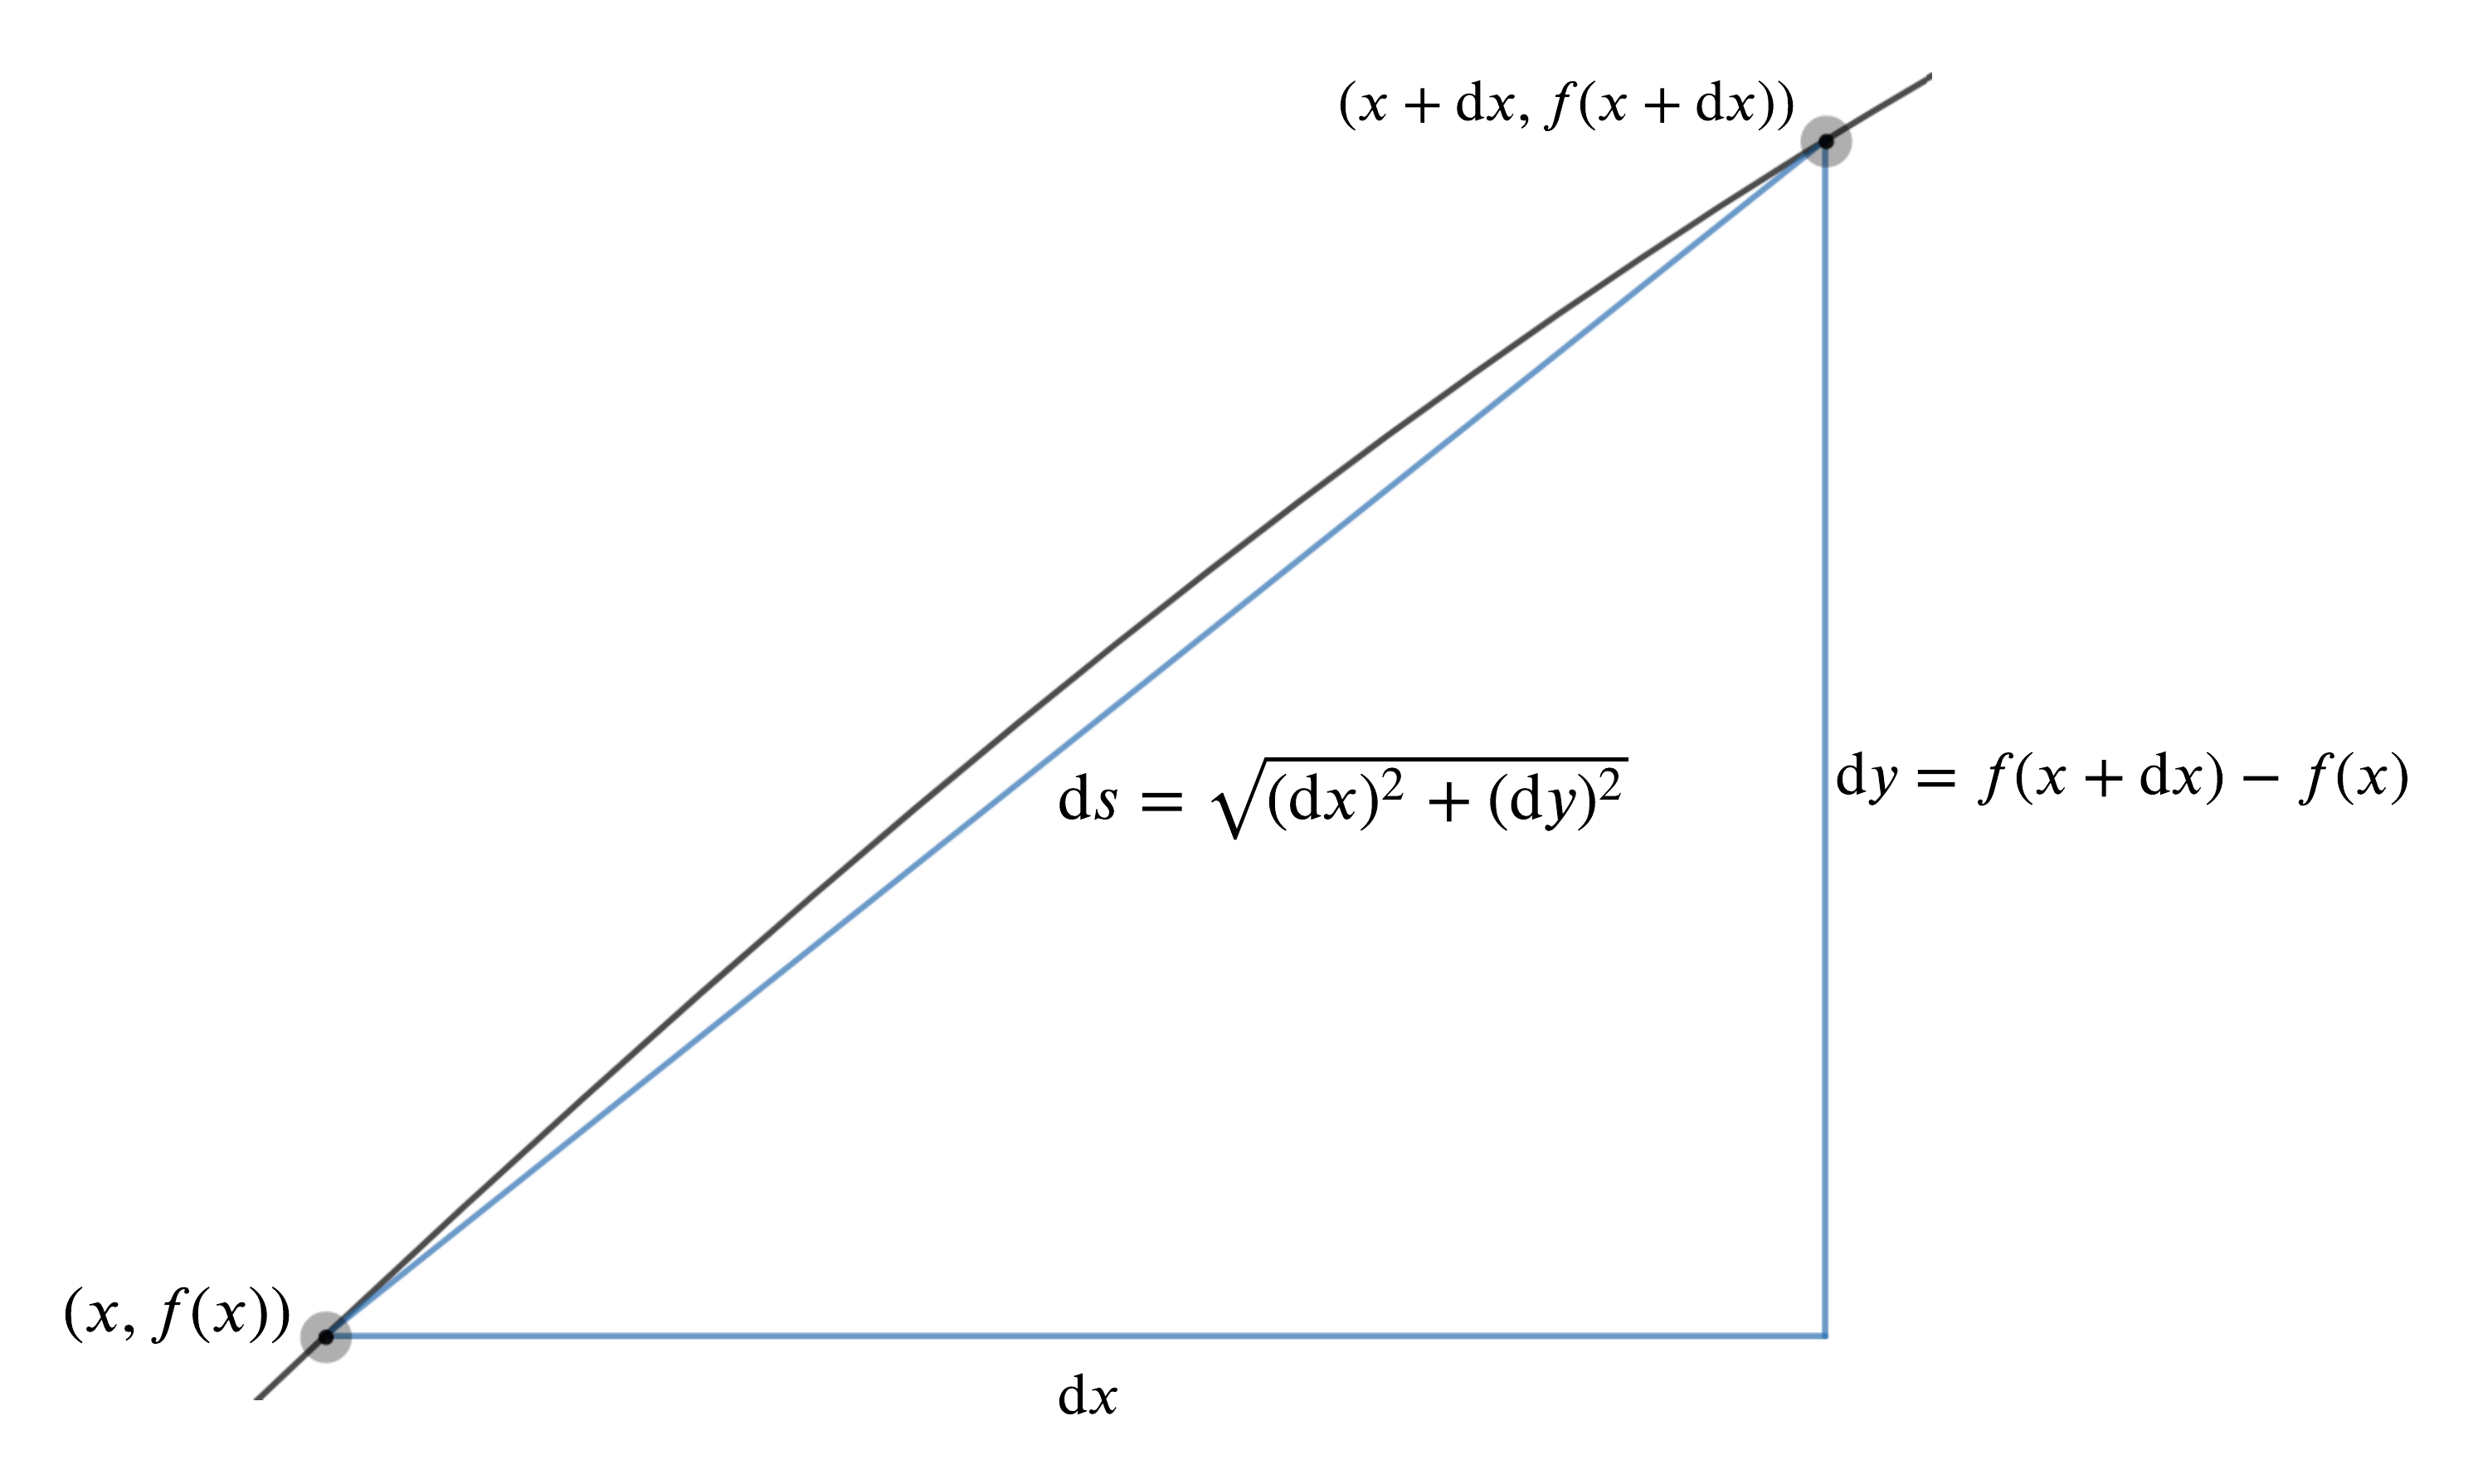
\includegraphics[width=0.66\textwidth]{./applications_integrals/arclength.png}
	\caption{\hyperref{}{}{}{Secant length approaches arc length}}
\end{figure}

As $\d{x}$ approaches 0, $\d{s}$, the length of the secant line, approaches the length of the curve.
If we summed all of these $\d{s}$'s in some interval we'd have the length of the curve on that interval.
\begin{align*}
	s &= \int_{a}^{b}{\d{s}} \\
	&= \int_{a}^{b}{\sqrt{(\d{x})^2+(\d{y})^2}} \\
	&= \int_{a}^{b}{\sqrt{(\d{x})^2\left(1+\left(\frac{\d{y}}{\d{x}}\right)^2\right)}} \\
	&= \int_{a}^{b}{\sqrt{1+\left(\frac{\d{y}}{\d{x}}\right)^2}\d{x}}.
\end{align*}

\begin{example}
	Show that the circumference of a circle with radius $r$ is $C=2\pi r$.
\end{example}
\begin{answer}
	Starting with the equation of a circle of radius $r$ and implicitly differentiating,
	\begin{align*}
		x^2 + y^2 &= r^2 \\
		2x + 2y\dd{y}{x} &= 0 \\
		\dd{y}{x} &= \frac{-x}{y} \\
		\left(\dd{y}{x}\right)^2 &= \frac{x^2}{y^2} = \frac{x^2}{r^2-x^2} \\
		C &= 2\int_{-r}^{r}{\sqrt{1+\frac{x^2}{r^2-x^2}}\d{x}} \\ 
		&\text{ (2 b/c we need to count upper and lower half)} \\
		&= 2\int_{-r}^{r}{\sqrt{\frac{r^2}{r^2-x^2}}\d{x}} \\
		&= 2\int_{-r}^{r}{r\sqrt{\frac{1}{r^2-x^2}}\d{x}} \\
		&= 2r\arcsin{\left(\frac{x}{r}\right)}\biggr\rvert_{-r}^{r} \\
		&= 2\pi r.
	\end{align*}
\end{answer}


Note that when deriving the arc length formula, we could have just as easily have divided by $(\d{y})^2$.
This would give us an equivalent arc length formula that's applicable when $x$ is a function of $y$.

\begin{example}
	Find the length of the curve $y=x^{1/3}$ from $(-8,2)$ to $(8,2)$.
\end{example}
\begin{answer}
	Rather than  tediously integrate the square root of a cube root if we set our bounds in terms of $x$, we can rewrite our equation and set out bounds in terms of $y$.
	\begin{align*}
		x &= y^3 \\
		\dd{x}{y} &= 3y^2 \\
		\left(\dd{x}{y}\right)^2 &= 9y^4 \\
		s &= \int_{-2}^{2}{\sqrt{1+9y^4}\d{y}} \\
		&\footnotemark\approx 17.261.
	\end{align*}
\end{answer}
\footnotetext{You shouldn't be expected to evaluate this integral analytically. Using a calculator to get a numerical answer is fine.}